\subsection{Izdelava krivulje}
Za operacijo odreza sem posebej izdelal krivuljo. Kot vzpona
sem zaokrožil na 150° in višino vzpona sem povečal na 15 mm,
kar pomeni, da sem moral uporabiti vzvod z razmerjem 1:5 na
sledilcu krivulje. Krivuljo sem izrisal in jo prenesel na
okrogel surovec iz jekla C45, premera 120 mm in debeline 8 mm, ki je imel
v sredini že izvrtano in postruženo luknjo premera 40 mm.
Potem sem na rezkalnem stroju z svedrom izvrtal luknje po obodu tako,
da se čim manj pokrivajo. Nekatere luknje mi ni uspelo natančno
izvrtati in se je po koncu vrtanja surovec še vedno držal skupaj
z krivuljo, katero sem z kladivom izbil. Na sliki \ref{izdelava_krivulje}
je prikazan ostanek surovca po vrtanju, ko sem izbil krivuljo.

\begin{figure}[H]
	\begin{center}
		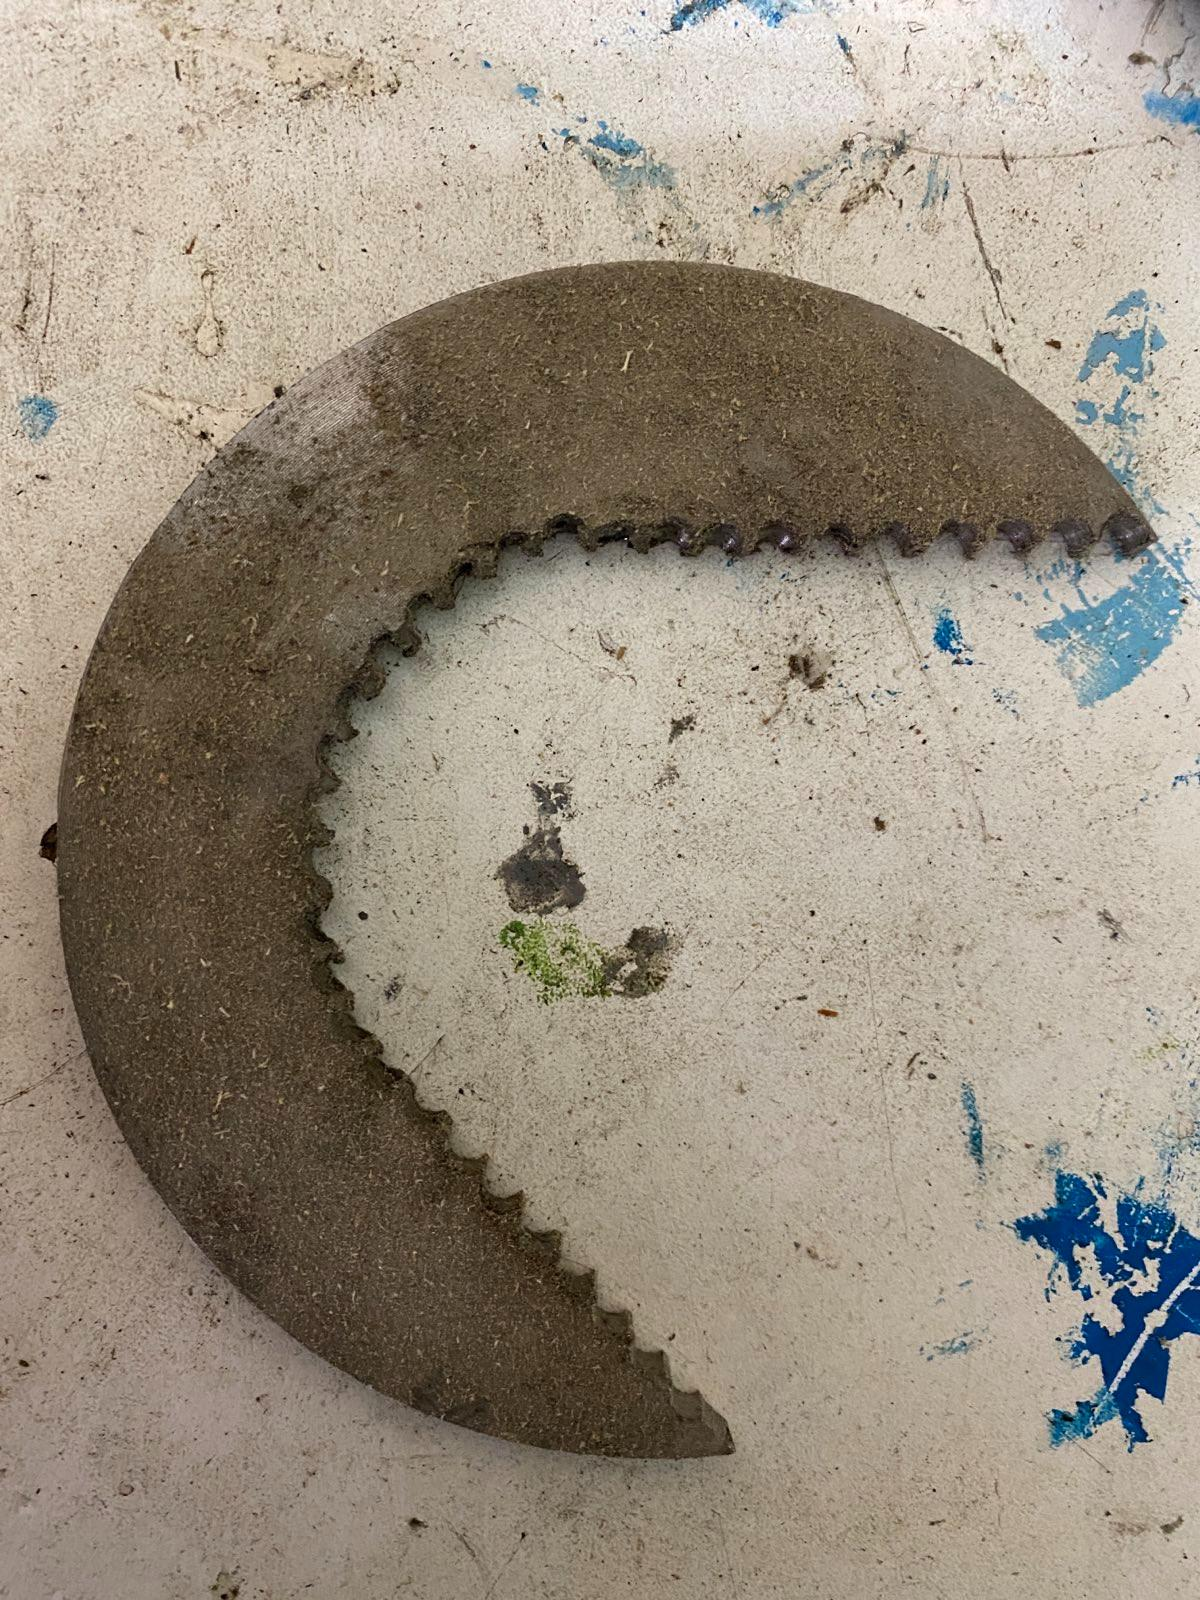
\includegraphics[width=6cm]{izdelava_krivulje.jpg}
		\caption{Ostanek surovca od vrtanja lukenj za izdelavo krivulje
			\cite{lasten}}
		\label{izdelava_krivulje}
	\end{center}
\end{figure}

Po tem sem krivuljo z ročno kotno brusilko izbrusil do vrisane linije
in izrezal sem še zarezo približno širine 35 mm, da se lahko krivulja
kasneje natakne na krivuljno gred in izdelava je bila skoraj zaključena.
Preostalo je še, da  krivuljo zakalim v kalilni peči, ter jo
še enkrat na fino pobrusim za čim bolj gladko površino,
da sledilec tem lepše potuje po njej.

Za kaljenje sem uporabil kalilno peč KAL 31, proizvajalca TerraArt
prikazana na \ref{kalilna_pec_slika}. Ta ima možnost programiranja
cikla segrevanja in nastavljanja hitrosti segrevanja in ohlajanja.

\begin{figure}[H]
	\begin{center}
		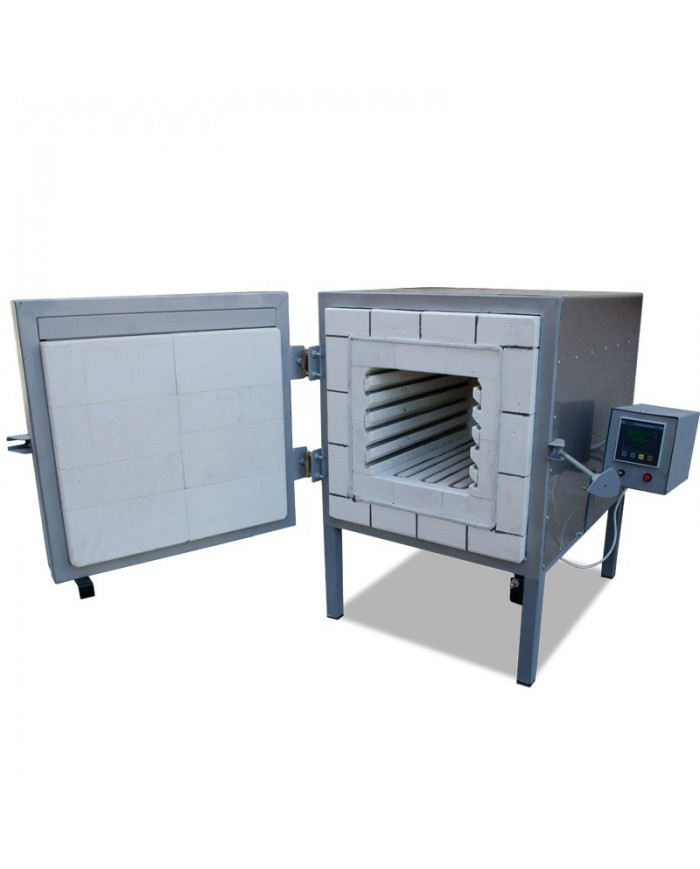
\includegraphics[width=8cm]{kalilna-pec-kal-31.jpg}
		\caption{Kalilna peč KAL 31
			\cite{kalilna_pec}}
		\label{kalilna_pec_slika}
	\end{center}
\end{figure}

Krivuljo sem po kaljenju zbrusil z ročno kotno brusilko in z tem
zaključil izdelavo. Preostalo je še, montaža na stroj in preizkus
delovanja. Če bi bilo potrebno karkoli popraviti, se lahko z
varilnim strojem navari tanjši sloj materiala in se ponovno zbrusi
površino. Krivulja bo po tem manj zdržala ampak je hitrejši postopek
popravljanja kot pa celoten postopek izdelave.
